% !TEX encoding = UTF-8 Unicode
\documentclass{article}[40pt]

\usepackage{ucs}
\usepackage{subcaption}
\usepackage{graphicx}
\usepackage{float}
\usepackage[utf8x]{inputenc}
\usepackage[greek,english]{babel}
\newcommand{\en}{\selectlanguage{english}}
\newcommand{\gr}{\selectlanguage{greek}}
\newcommand{\es}{\textsuperscript{\gr es}}
\usepackage{xspace}
\usepackage{amssymb}
\usepackage[colorlinks]{hyperref}
\usepackage[fleqn]{mathtools}
%\usepackage[fleqn]{amsmath}
\usepackage[export]{adjustbox}
\usepackage{subcaption}
\usepackage{xcolor}
\usepackage{listings}
\hypersetup{
    colorlinks=true,% make the links colored
}


\definecolor{mGreen}{rgb}{0,0.6,0}
\definecolor{mGray}{rgb}{0.5,0.5,0.5}
\definecolor{mPurple}{rgb}{0.58,0,0.82}
\definecolor{backgroundColour}{rgb}{255,255,255}
\lstdefinestyle{PStyle}{
    backgroundcolor=\color{backgroundColour},   
    commentstyle=\color{mGreen},
    keywordstyle=\color{magenta},
    numberstyle=\tiny\color{mGray},
    stringstyle=\color{mPurple},
    basicstyle=\footnotesize,
    breakatwhitespace=false,         
    breaklines=true,                 
    captionpos=b,                    
    keepspaces=true,                 
    numbers=left,                    
    numbersep=5pt,                  
    showspaces=false,                
    showstringspaces=false,
    showtabs=false,                  
    tabsize=2,
    basicstyle=\fontsize{7}{9}\selectfont\ttfamily,
	xleftmargin=0.25\textwidth,
    language=Python
}



\title{\gr \gr ΠΑΝΕΠΙΣΤΗΜΙΟ ΙΩΑΝΝΙΝΩΝ \\ ΤΜΗΜΑ ΜΗΧΑΝΙΚΩΝ Η/Υ  \&  ΠΛΗΡΟΦΟΡΙΚΗΣ \\ \gr ΜΥΕ002 - ΜΗΧΑΝΙΚΗ ΜΑΘΗΣΗ \\ ΑΣΚΗΣΗ 1}
\author{\gr Κίτσιος Κωνσταντίνος 4388 \\\gr Λιόντος Αναστάσιος 4409}
\begin{document}
\maketitle
\newpage
\hypersetup{linkcolor=black}
\tableofcontents
\newpage
\section{\gr Μέθοδος \en K-nearest neighbours.}
\begin{lstlisting}[style=PStyle]
import idx2numpy as idx2numpy
import numpy as np
import pandas
import matplotlib.pyplot as plt
from sklearn.neighbors import KNeighborsClassifier
from sklearn import metrics
from Resize import resize


trainImagePath = "../dataset/train-images-idx3-ubyte"
trainLabelPath = "../dataset/train-labels-idx1-ubyte"
testImagePath = "../dataset/t10k-images-idx3-ubyte"
testLabelPath="../dataset/t10k-labels-idx1-ubyte"

x_train = idx2numpy.convert_from_file(trainImagePath)
y_train = idx2numpy.convert_from_file(trainLabelPath)

x_test = idx2numpy.convert_from_file(testImagePath)
y_test = idx2numpy.convert_from_file(testLabelPath)

x_train=resize(x_train,28,28,7,7)
x_test=resize(x_test,28,28,7,7)

x_train=x_train.reshape((x_train.shape[0], 7*7))
x_test=x_test.reshape((x_test.shape[0], 7*7))

x_train=x_train/255.0
x_test=x_test/255.0

k=[1,5,10]
accuracy=[]
F1score=[]
for i in k:
     knn=KNeighborsClassifier(n_neighbors=i, metric="cosine")
     knn.fit(x_train,y_train)
     y_pred=knn.predict(x_test)
     accuracy.append(metrics.accuracy_score(y_test, y_pred))
     F1score.append(metrics.f1_score(y_true=y_test, y_pred=y_pred, average='macro'))

print(15*'-'+'cosine distance'+15*'-')
for i in range(3):
     print("k={}: [acc={:.3f}%]".format(k[i],accuracy[i]*100.0), end="  ")
     print()
     print("k={}: [f1 score={:.3f}%]".format(k[i],F1score[i]*100.0), end="  ")
     if i!=2: print("\n-----------------------")
     else: print()

accuracy=[]
F1score=[]
for i in k:
     knn=KNeighborsClassifier(n_neighbors=i,metric='minkowski', p=2)
     knn.fit(x_train,y_train)
     y_pred=knn.predict(x_test)
     accuracy.append(metrics.accuracy_score(y_test, y_pred))
     F1score.append(metrics.f1_score(y_true=y_test, y_pred=y_pred, average='macro'))
print(15*'-'+'euclidean distance'+15*'-')
for i in range(3):
     print("k={}: [acc={:.3f}%]".format(k[i],accuracy[i]*100.0), end="  ")
     print()
     print("k={}: [f1 score={:.3f}%]".format(k[i],F1score[i]*100.0), end="  ")
     if i!=2: print("\n-----------------------")
     else: print()
\end{lstlisting}
\gr Στη μέθοδο \en K-nearest neighbours \gr φορτώνουμε τα σύνολα εκπαίδευσης και δοκιμής. Στη συνέχεια ορίζουμε έναν πίνακα \en k \gr που αναπαριστά τον αριθμό των ζητούμενων γειτόνων. Έπειτα, δημιουργούμε το μοντέλο με παραμέτρους την ευκλείδια απόσταση τον αριθμό γειτόνων όπου ζητείται στην εκφώνηση και τέλος το εκπαιδεύουμε και αξιολογούμε το μοντέλο με το σύνολο δοκιμής, με τα στατιστικά \en accuracy \& F1 Score \gr. Παρόμοια διαδικασία εκτελούμε και για την συνημιτονοειδή απόσταση. Τα αποτελέσματα της μεθόδου \en KNN \gr για τις ζητούμενες αποστάσεις είναι τα εξής:\en
\begin{lstlisting}
-----------------------Cosine Distance-----------------------
k=1: [Accuracy=84.070%]  
k=1: [F1 score=84.072%]
------------------------  
k=5: [Accuracy=85.370%]  
k=5: [F1 score=85.223%]
-----------------------  
k=10: [Accuracy=84.880%]  
k=10: [F1 score=84.682%]  
-----------------------Euclidean distance-----------------------
k=1: [Accuracy=82.950%]  
k=1: [F1 score=83.013%]
-----------------------  
k=5: [Accuracy=84.170%]  
k=5: [F1 score=84.030%]
-----------------------  
k=10: [Accuracy=84.190%]  
k=10: [F1 score=84.027%]
\end{lstlisting}\newpage
\section{\gr Μέθοδος \en Support Vector Machines (SVM).}
\begin{lstlisting}[style=PStyle]
import idx2numpy
import numpy as np
import matplotlib.pyplot as plt
import random
from sklearn import svm, metrics
import sklearn
from Resize import resize
from math import pow
trainImagePath = "../dataset/train-images-idx3-ubyte"
trainLabelPath = "../dataset/train-labels-idx1-ubyte"
testImagePath = "../dataset/t10k-images-idx3-ubyte"
testLabelPath="../dataset/t10k-labels-idx1-ubyte"

x_test = idx2numpy.convert_from_file(trainImagePath)
y_test = idx2numpy.convert_from_file(trainLabelPath)

x_train = idx2numpy.convert_from_file(testImagePath)
y_train = idx2numpy.convert_from_file(testLabelPath)

resize(x_train,28,28,7,7)
resize(x_test,28,28,7,7)



x_train=x_train.reshape((x_train.shape[0], 7*7))
x_test=x_test.reshape((x_test.shape[0], 7*7))

x_train=x_train/255.0
x_test=x_test/255.0

linear=svm.SVC(kernel='linear',C=1,decision_function_shape='ovr').fit(x_train,y_train)
sigmoid=svm.SVC(kernel='sigmoid',C=1,decision_function_shape='ovr').fit(x_train,y_train)
x_train = x_train.astype('float32')
cosine=svm.SVC(kernel=sklearn.metrics.pairwise.cosine_similarity,C=1,decision_function_shape='ovr').fit(x_train,y_train)

lpred=linear.predict(x_test)
sigpred=sigmoid.predict(x_test)
cospred=cosine.predict(x_test)


print("Linear Kernel")
print("{:.3f}".format(metrics.accuracy_score(y_test, lpred)*100.0))
print("{:.3f}".format(metrics.f1_score(y_true=y_test, y_pred=lpred, average='macro')*100.0))
print("Sigmoid Kernel")
print("{:.3f}".format(metrics.accuracy_score(y_test, sigpred)*100.0))
print("{:.3f}".format(metrics.f1_score(y_true=y_test, y_pred=sigpred, average='macro')*100.0))
print("Cosine Kernel")
print("{:.3f}".format(metrics.accuracy_score(y_test, cospred)*100.0))
print("{:.3f}".format(metrics.f1_score(y_true=y_test, y_pred=cospred, average='macro')*100.0))
\end{lstlisting}
\gr Στη μέθοδο \en Support Vector Machines \gr φορτώνουμε τα σύνολα εκπαίδευσης και δοκιμής. Έπειτα, δημιουργούμε το μοντέλο για κάθε συνάρτηση πυρήνα όπου ζητείται στην εκφώνηση, χρησιμοποιώντας την στρατηγική \en one-versus-all \gr και τέλος το εκπαιδεύουμε και αξιολογούμε το μοντέλο με το σύνολο δοκιμής, με τα στατιστικά \en accuracy \& F1 Score \gr. Τα αποτελέσματα της μεθόδου \en SVM \gr για τις ζητούμενες συναρτήσεις πυρήνα είναι τα εξής:\en
\begin{lstlisting}
Linear Kernel
Accuracy = 79.577%
F1 Score = 79.063%

Sigmoid Kernel
Accuracy = 31.342%
F1 Score = 30.816%

Cosine Kernel
Accuracy = 80.272%
F1 Score = 79.653%
\end{lstlisting}\newpage
\section{\gr Μέθοδος \en Neural Networks.}
\begin{lstlisting}[style=PStyle]
import idx2numpy
# TensorFlow and tf.keras
import tensorflow as tf

# Helper libraries
import numpy as np
import matplotlib.pyplot as plt
from sklearn import metrics
import Resize

trainImagePath = "../dataset/train-images-idx3-ubyte"
trainLabelPath = "../dataset/train-labels-idx1-ubyte"
testImagePath = "../dataset/t10k-images-idx3-ubyte"
testLabelPath="../dataset/t10k-labels-idx1-ubyte"

x_train = idx2numpy.convert_from_file(trainImagePath)
y_train = idx2numpy.convert_from_file(trainLabelPath)

x_test = idx2numpy.convert_from_file(testImagePath)
y_test = idx2numpy.convert_from_file(testLabelPath)


x_train = x_train / 255.0
x_test = x_test / 255.0

x_test=x_test.reshape((x_test.shape[0], 28*28))

model = tf.keras.Sequential([
   tf.keras.layers.Flatten(input_shape=(28,28)),
   tf.keras.layers.Dense(500, activation='sigmoid'),
   tf.keras.layers.Dense(10)
])

model.compile(optimizer='sgd',
               loss=tf.keras.losses.SparseCategoricalCrossentropy(from_logits=True))
model.fit(x_train, y_train, epochs=10)


probability_model = tf.keras.Sequential([model,tf.keras.layers.Softmax()])
prediction = probability_model.predict(x_test)

predictions=[]
for i in range(prediction.shape[0]):
   predictions.append(np.argmax(prediction[i]))
print("One hidden layer")
print("acc={:.3f}%".format(metrics.accuracy_score(y_test, predictions)*100.0))
print("f1 score={:.3f}%".format(metrics.f1_score(y_true=y_test, y_pred=predictions, average='macro')*100.0))


model = tf.keras.Sequential([
    tf.keras.layers.Flatten(input_shape=(28, 28)),
    tf.keras.layers.Dense(500, activation='sigmoid'),
    tf.keras.layers.Dense(200, activation='sigmoid'),
    tf.keras.layers.Dense(10)
])

model.compile(optimizer='sgd',
                loss=tf.keras.losses.SparseCategoricalCrossentropy(from_logits=True))
model.fit(x_train, y_train, epochs=10)


probability_model = tf.keras.Sequential([model,tf.keras.layers.Softmax()])
prediction = probability_model.predict(x_test)

predictions=[]
for i in range(prediction.shape[0]):
    predictions.append(np.argmax(prediction[i]))
print("Two hidden layers")
print("acc={:.3f}%".format(metrics.accuracy_score(y_test, predictions)*100.0))
print("f1 score={:.3f}%".format(metrics.f1_score(y_true=y_test, y_pred=predictions, average='macro')*100.0))
\end{lstlisting}
\gr\gr Στη μέθοδο \en Neural Networks \gr φορτώνουμε τα σύνολα εκπαίδευσης και δοκιμής. Έπειτα, δημιουργούμε το μοντέλο, πρώτα για ένα κρυμμένο επίπεδο με 500 κρυμμένους νευρώνες και έπειτα για δύο κρυμμένα επίπεδα και με 500 κρυμμένους νευρώνες στο πρώτο επίπεδο και 200 στο δεύτερο. Τέλος το εκπαιδεύουμε και αξιολογούμε το μοντέλο με το σύνολο δοκιμής χρησιμοποιώντας τη μέθοδο βελτιστοποίσης \en Stochastic Gradient Descent, \gr με τα στατιστικά \en accuracy \& F1 Score. \gr Η εξόδος του δικτύου αποτελείται από 10 νευρώνες και χρησιμοποιώντας τη συνάρτηση ενεργοποίησης \en softmax \gr, υπολογίζουμε την πιθανότητα να ανήκει ένα δεδομένο (εικόνα) σε κάθε μια κατηγορία. Τα αποτελέσματα της μεθόδου \en Neural Networks \gr για τα ζητούμενα κρυμμένα επίπεδα είναι τα εξής:\en
\begin{lstlisting}
One hidden layer
Epoch 1/10
1875/1875 [==============================] - 4s 2ms/step - loss: 1.1632
Epoch 2/10
1875/1875 [==============================] - 4s 2ms/step - loss: 0.7121
Epoch 3/10
1875/1875 [==============================] - 4s 2ms/step - loss: 0.6231
Epoch 4/10
1875/1875 [==============================] - 4s 2ms/step - loss: 0.5766
Epoch 5/10
1875/1875 [==============================] - 4s 2ms/step - loss: 0.5465
Epoch 6/10
1875/1875 [==============================] - 4s 2ms/step - loss: 0.5247
Epoch 7/10
1875/1875 [==============================] - 4s 2ms/step - loss: 0.5086
Epoch 8/10
1875/1875 [==============================] - 4s 2ms/step - loss: 0.4959
Epoch 9/10
1875/1875 [==============================] - 4s 2ms/step - loss: 0.4854
Epoch 10/10
1875/1875 [==============================] - 4s 2ms/step - loss: 0.4763
Accuracy=82.100%
F1 score=81.854%

Two hidden layers
Epoch 1/10
1875/1875 [==============================] - 5s 3ms/step - loss: 1.8323
Epoch 2/10
1875/1875 [==============================] - 5s 3ms/step - loss: 1.0929
Epoch 3/10
1875/1875 [==============================] - 6s 3ms/step - loss: 0.8415
Epoch 4/10
1875/1875 [==============================] - 5s 3ms/step - loss: 0.7268
Epoch 5/10
1875/1875 [==============================] - 6s 3ms/step - loss: 0.6674
Epoch 6/10
1875/1875 [==============================] - 5s 3ms/step - loss: 0.6304
Epoch 7/10
1875/1875 [==============================] - 5s 3ms/step - loss: 0.6029
Epoch 8/10
1875/1875 [==============================] - 5s 3ms/step - loss: 0.5801
Epoch 9/10
1875/1875 [==============================] - 5s 3ms/step - loss: 0.5616
Epoch 10/10
1875/1875 [==============================] - 5s 3ms/step - loss: 0.5449
Accuracy=79.690%
F1 score=79.484%
\end{lstlisting}\newpage
\section{\gr Μέθοδος \en Naive Bayes Classifier.}
\begin{lstlisting}[style=PStyle]
from math import sqrt, exp, pi, pow
import idx2numpy
from sklearn import metrics
from Resize import resize
#Calculate mean.
def mean(numbers):
	return sum(numbers)/float(len(numbers)) if sum(numbers)/float(len(numbers)) !=0 else pow(10,-20)

 #Calculate the standard deviation of a list of numbers
def stdev(numbers):
	avg = mean(numbers)
	variance = sum([pow(x-avg,2) for x in numbers])/float(len(numbers)-1)
	return sqrt(variance)

# Split the dataset by class values, returns a dictionary
def separate_by_class(X,Class):
	separated = dict()
	for i in range(len(X)):
		vector = X[i]
		class_value = Class[i]

		if (class_value not in separated):
			separated[class_value] = list()
		separated[class_value].append(vector)
	return separated

# Calculate the mean, stdev and count for each column in a dataset
def summarize_dataset(dataset):
	summaries = [(mean(column), stdev(column), len(column)) for column in zip(*dataset)]
	del(summaries[-1])
	return summaries

# Split dataset by class then calculate statistics for each row
def fit(X,Class):
    summaries = dict()
    seperated = separate_by_class(X,Class);
    for class_value, rows in seperated.items():
        summaries[class_value] = summarize_dataset(rows)
    return summaries

# Calculate the Gaussian probability distribution function for x
def calculate_probability(x, mean, stdev):
	exponent = exp(-((x-mean)**2 / (2 * stdev**2 )))
	return (1 / (sqrt(2 * pi) * stdev)) * exponent
 
# Calculate the probabilities of predicting each class for a given row
def calculate_class_probabilities(summaries, row):
	total_rows = sum([summaries[label][0][2] for label in summaries])
	probabilities = dict()
	for class_value, class_summaries in summaries.items():
		probabilities[class_value] = summaries[class_value][0][2]/float(total_rows)
		for i in range(len(class_summaries)):
			mean, stdev, _ = class_summaries[i]
			probabilities[class_value] *= calculate_probability(row[i], mean, stdev)
	return probabilities
 
# Predict the class for a given row
def predict(summaries, row):	
	predictions=list()
	for i in range(len(row)):
		probabilities = calculate_class_probabilities(summaries, row[i])
		best_label, best_prob = None, -1
		for class_value, probability in probabilities.items():
			if best_label is None or probability > best_prob:
				best_prob = probability
				best_label = class_value
		predictions.append(best_label)		
	return predictions    


#Main
trainImagePath = "../dataset/train-images-idx3-ubyte"
trainLabelPath = "../dataset/train-labels-idx1-ubyte"
testImagePath = "../dataset/t10k-images-idx3-ubyte"
testLabelPath="../dataset/t10k-labels-idx1-ubyte"

x_train = idx2numpy.convert_from_file(trainImagePath)
y_train = idx2numpy.convert_from_file(trainLabelPath)

x_test = idx2numpy.convert_from_file(testImagePath)
y_test = idx2numpy.convert_from_file(testLabelPath)

x_train=resize(x_train,28,28,7,7)
x_test=resize(x_test,28,28,7,7)



x_train=x_train.reshape((x_train.shape[0], 7 * 7))
x_test=x_test.reshape((x_test.shape[0], 7*7))

x_train=x_train/255.0
x_test=x_test/255.0

model = fit(x_train,y_train)

predictions=predict(model,x_test)
print("{:.3f}".format(metrics.accuracy_score(y_test, predictions)*100.0))
print("{:.3f}".format(metrics.f1_score(y_true=y_test, y_pred=predictions, average='macro')*100.0))
\end{lstlisting}
\gr Στη μέθοδο \en Naive Bayes Classifier \gr υλοποιούμε τις μεθόδους \en mean \& stdev \gr οι οποίες υπολογίζουν τη μέση τιμή και την τυπική απόκλιση. Στη συνέχεια η μέθοδος \en seperate\_by\_class \gr η οποία επιστρέφει ένα λεξικό στο οποίο το κλειδί είναι η κλαση της εικόνας και τιμή όλες τις εικόνες που ανήκουν σε αυτή την κλάση. Η μέθοδος \en summarize\_class \gr υπολογίζει τη μέση τιμή και τυπική απόκλιση για κάθε στήλη, κάθε εικόνας του συνόλου δεδομένων. Η μέθοδος \en calculate\_class\_probabilities \gr υπολογίζει τις πιθανότητες πρόβλεψης κάθε κλάσης για μία δεδομένη εικόνα, χρησιμοποιώντας τη βοηθητική μέθοδο \en calculate\_probability \gr η οποία υπολογίζει την γκαουσιανή πιθανότητα ενός αριθμού. Για την εκπαίδευση και πρόβλεψη του μοντέλου, υπολοιποιούμε τις μεθόδους \en fit \& predict \gr αντίστοιχα. Τέλος αξιολογούμε το μοντέλο με τα στατιστικά \en accuracy \& F1 Score.\gr Τα αποτελέσματα της μεθόδου \en Naive Bayes Classifier \gr είναι τα εξής:\en
\begin{lstlisting}
Accuracy=60.070%
F1 score=57.285%
\end{lstlisting}\newpage
\section{\gr Βοηθητική μέθοδος \en resize.}
\gr Στις παραπάνω μεθόδους, χρησιμοποιήσαμε μία βοηθητική μέθοδο \en resize \gr, η οποία επαναπροσδιορίζει το μέγεθος της κάθε εικόνας σε \en pixels. \gr Η μέθοδος παίρνει σαν όρισμα το σύνολο δεδομένων, τις αρχικές διαστάσεις της κάθε εικόνας και τις διαστάσεις που επιθυμούμε για να επαναπροσδιορίσουμε το μέγεθος.
\section{\gr Βέλτιστη μέθοδος}
\gr Έπειτα από σύγκριση των αποτελεσμάτων \en Accuracy, F1 Score \gr καταλήγουμε πως η βέλτιση μέθοδος ταξινόμησης είναι αυτή της μεθόδου \en K-nearest neighbours \gr με συνημιτονοειδή απόσταση και \en $k=5$ \gr γείτονες. Στα γράφημα που ακολουθεί, φαίνεται το ποσοστό επιτυχίας και το \en F1 Score \gr για την κάθε μέθοδο που υλοποιήσαμε.\\\\ \en
\begin{figure}[!htpb]
\centering
  \begin{minipage}[b]{1\textwidth}
    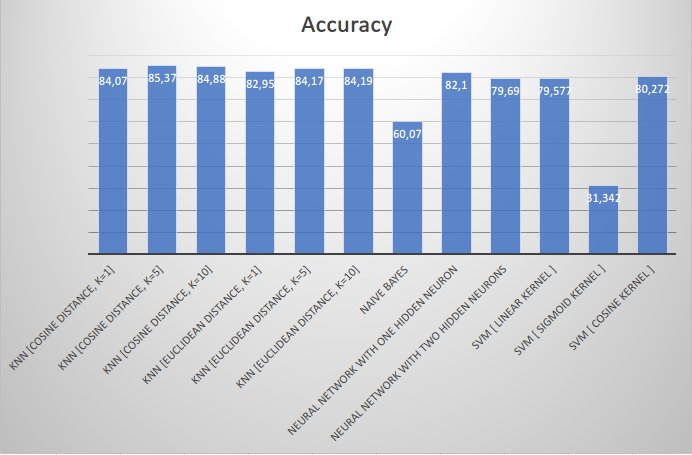
\includegraphics[width=1\linewidth]{accuracy.png}
    \label{fig:1}
  \end{minipage}
  \quad
  \begin{minipage}[b]{1\textwidth}
    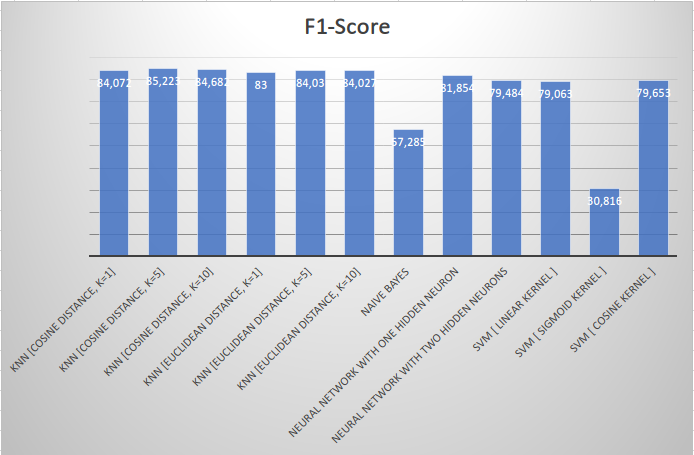
\includegraphics[width=1\linewidth]{f1score.png}
  \end{minipage}
\end{figure}
\end{document}
